% Teaser: TikZ. Values are real: sakila_1 film table (A = AVG(rental_rate / rental_duration), B = AVG(rental_rate) /
% AVG(rental_duration), per rating). Model outcomes are the recorded single-call responses to the open film request
% (out/transfer/eval12-v2/render/disclose/*/...06768b2b94__open.json).
% Shared setup for the diagrams (teaser, pipeline, worked). Built with XeLaTeX so that all text is Arial, in black.
% Sizes match the paper's acmart sigconf sizes (\footnotesize 7 pt); the smallest text is 6 pt.
\documentclass[border=0.5pt]{standalone}
\usepackage{fontspec}
\setmainfont{Arial}\setsansfont{Arial}\setmonofont{Menlo}[Scale=MatchLowercase]
\usepackage{unicode-math}\setmathfont{FiraMath-Regular.otf}
\usepackage{booktabs}
\usepackage{tikz}
\usetikzlibrary{arrows.meta,calc,positioning,fit,backgrounds,shapes.geometric}
\renewcommand\large{\fontsize{10}{12}\selectfont}
\renewcommand\small{\fontsize{8}{10}\selectfont}
\renewcommand\footnotesize{\fontsize{7}{8.4}\selectfont}
\renewcommand\scriptsize{\fontsize{6.5}{7.6}\selectfont}
\renewcommand\tiny{\fontsize{6}{7}\selectfont}
\newcommand{\nohyph}{\hyphenpenalty=10000\exhyphenpenalty=10000\relax}
\newcommand{\sql}[1]{\texttt{#1}}
% the edited SQL clause, highlighted as in AMBROSIA and the test-suite paper; plain check and cross marks
\newcommand{\hl}[2]{{\setlength{\fboxsep}{0.7pt}\colorbox{#1f}{\vphantom{Ay}\texttt{#2}}}}
\newfontfamily\markfont{Arial Unicode MS}\newcommand{\yes}{{\markfont ✓}}\newcommand{\no}{{\markfont ✗}}
% math letters in Arial italic; the open-request circle is drawn; only the arrow comes from Fira Math
\newcommand{\vq}[1]{\textit{q}\textsubscript{#1}}\newcommand{\vp}[1]{\textit{p}\textsubscript{#1}}\newcommand{\vo}{\mbox{\textit{q}\hspace{0.3pt}\raisebox{-0.25ex}{\tikz[baseline=0pt]\draw[line width=0.45pt] (0,1.1pt) circle (1.1pt);}}}
% box lines: A (blue) and B (orange) as in the data figures; neutral lines grey. Text is always black.
% colors as in AMBROSIA's and AmbiQT's diagrams (draw.io palette): interpretation A blue, interpretation B orange, code blocks light gray
\definecolor{sbA}{HTML}{6C8EBF}\definecolor{sbB}{HTML}{D79B00}\definecolor{sbAf}{HTML}{DAE8FC}\definecolor{sbBf}{HTML}{FFE6CC}\definecolor{sbline}{HTML}{4D4D4D}
\definecolor{sbfill}{HTML}{F5F5F5}

\begin{document}
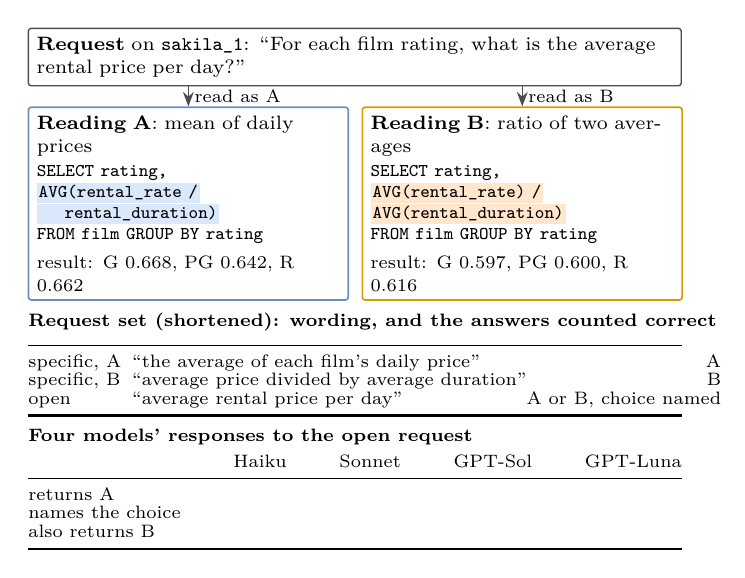
\begin{tikzpicture}[x=1cm, y=1cm, font=\footnotesize, >=Stealth, line width=0.5pt,
  rd/.style={draw=#1, line width=0.6pt, rounded corners=1pt, inner sep=3pt, align=left, text width=3.85cm, anchor=north west},
  arr/.style={->, draw=sbline},
  lab/.style={font=\scriptsize\bfseries, text=black, anchor=west, inner sep=0pt}]
% ---- 1 the request
\node[draw=sbline, rounded corners=1pt, inner sep=3pt, text width=8.08cm, align=left, anchor=north west] (q) at (0,0)
  {\textbf{Request} on \texttt{sakila\_1}: ``For each film rating, what is the average rental price per day?''};
% ---- 2 two correct readings: complete SQL (the part that differs highlighted) and the result
\node[rd=sbA] (A) at (0,-1.0) {\textbf{Reading A}: mean of daily prices\\[1pt]\scriptsize
  \texttt{SELECT rating,}\\\hl{sbA}{AVG(rental\_rate /}\\\hl{sbA}{\ \ \ \ rental\_duration)}\\\texttt{FROM film GROUP BY rating}\\[2pt]
  result: G 0.668, PG 0.642, R 0.662};
\node[rd=sbB] (B) at (4.24,-1.0) {\textbf{Reading B}: ratio of two averages\\[1pt]\scriptsize
  \texttt{SELECT rating,}\\\hl{sbB}{AVG(rental\_rate) /}\\\hl{sbB}{AVG(rental\_duration)}\\\texttt{FROM film GROUP BY rating}\\[2pt]
  result: G 0.597, PG 0.600, R 0.616};
\draw[arr] (A.north |- q.south) -- node[right, font=\scriptsize, inner sep=2pt] {read as A} (A.north);
\draw[arr] (B.north |- q.south) -- node[right, font=\scriptsize, inner sep=2pt] {read as B} (B.north);
% ---- 3 the request set: the same request written three ways
\node[lab, anchor=north west] (l1) at ([yshift=-4pt]A.south west) {Request set (shortened): wording, and the answers counted correct};
\node[anchor=north west, inner sep=0pt] (t1) at ([yshift=-3pt]l1.south west) {\scriptsize\setlength{\tabcolsep}{0pt}\renewcommand{\arraystretch}{0.88}%
\begin{tabular*}{8.3cm}{@{\extracolsep{\fill}}l@{\hspace{4pt}}lr@{}}
\midrule
specific, A & ``the average of each film's daily price'' & A\\
specific, B & ``average price divided by average duration'' & B\\
open & ``average rental price per day'' & A or B, choice named\\\bottomrule
\end{tabular*}};
% ---- 4 what four models did with the open request
\node[lab, anchor=north west] (l2) at ([yshift=-4pt]t1.south west) {Four models' responses to the open request};
\node[anchor=north west, inner sep=0pt] at ([yshift=-3pt]l2.south west) {\scriptsize\setlength{\tabcolsep}{0pt}\renewcommand{\arraystretch}{0.88}%
\begin{tabular*}{8.3cm}{@{\extracolsep{\fill}}lcccc@{}}
 & Haiku & Sonnet & GPT-Sol & GPT-Luna\\\midrule
returns A & \yes & \yes & \yes & \yes\\
names the choice & \no & \yes & \no & \yes\\
also returns B & \no & \yes & \no & \no\\\bottomrule
\end{tabular*}};
\end{tikzpicture}
\end{document}
